%---------------------------------------------------------------------
%
%                          Cap�tulo 5
%
%---------------------------------------------------------------------
%
% 05Bibliografia.tex
% Copyright 2009 Marco Antonio Gomez-Martin, Pedro Pablo Gomez-Martin
%
% This file belongs to the TeXiS manual, a LaTeX template for writting
% Thesis and other documents. The complete last TeXiS package can
% be obtained from http://gaia.fdi.ucm.es/projects/texis/
%
% Although the TeXiS template itself is distributed under the 
% conditions of the LaTeX Project Public License
% (http://www.latex-project.org/lppl.txt), the manual content
% uses the CC-BY-SA license that stays that you are free:
%
%    - to share & to copy, distribute and transmit the work
%    - to remix and to adapt the work
%
% under the following conditions:
%
%    - Attribution: you must attribute the work in the manner
%      specified by the author or licensor (but not in any way that
%      suggests that they endorse you or your use of the work).
%    - Share Alike: if you alter, transform, or build upon this
%      work, you may distribute the resulting work only under the
%      same, similar or a compatible license.
%
% The complete license is available in
% http://creativecommons.org/licenses/by-sa/3.0/legalcode
%
%---------------------------------------------------------------------

\chapter{Pruebas con usuarios}
\label{cap5}
\label{cap:pruebas}

En el cap\'itulo anterior hemos visto c\'omo se ha realizado la implementaci\'on de las diferentes caracter\'iticas de la aplicaci\'on de Android y Unity. Adem\'as de esto, se han explicado cada una de las clases que contiene la librar\'ia y de las que deber\'a hacer uso el desarrollador.\\
En este cap\'itulo se va explicar la integraci\'on de la librer\'ia en un proyecto ya terminado. Este proyecto ha sido sacado de la \textit{Unity Asset Store}\footnote{https://assetstore.unity.com/} y se va a utilizar para realizar pruebas de rendimiento de la librer\'ia. Estas pruebas se realizar\'an con usuarios ajenos al proyecto y los resultados marcaran los aspectos a mejorar en futuras revisiones de este trabajo. \\

%-------------------------------------------------------------------
\section{Integraci\'on de la librer\'ia en juegos finalizados}
%-------------------------------------------------------------------

Unity ofrece una plataforma de aprendizaje llamada \textbf{\textit{Unity Learn}}.\footnote{https://learn.unity.com/projects} En esta plataforma se encuentran varios proyectos en los cuales pueden incluirse diferentes modificaciones explicadas en la propia plataforma para aprender a utilizar algunos aspectos de Unity. El proyecto escogido de la plataforma ha sido \textbf{Karting Microgame}\footnote{https://assetstore.unity.com/packages/templates/karting-microgame-150956?}, un juego de conducci\'on arcade muy parecido a la saga de \textbf{\textit{Mario Kart}} desarrollada por Nintendo.\\

Este proyecto desarrollado por los trabajadores de Unity ha sido el utilizado para probar la librer\'ia que se ha desarrollado en este proyecto. El objetivo de integrar la librer\'ia en un juego terminado es el de probar c\'omo de f\'acil es utilizar la herramienta desarrollada en este trabajo. Adem\'as, una vez est\'e integrada en el juego se realizaran una serie de purebas de rendimiento con usuarios. Los usuarios utilizar\'an la librer\'ia para jugar mientras que se est\'an monitorizando sus acciones. Como se explic\'o en el cap\'itulo anterior, el dispositivo m\'ovil necesita conocer la IP y el puerto del juego para poder establecer una conexi\'on. Esto se realiza mediante un c\'odigo QR cuya implementaci\'on no viene incluida en la librer\'ia ya que esta es una soluci\'on que se ha propuesto para este ejemplo.\\

Esta implementaci\'on del c\'odigo QR utiliza la librer\'ia \textbf{ZXing} en su versi\'on de .NET. En la soluci\'on propuesta, la clase que se encarga del manejo del QR tambi\'en se encarga de obtener la IP del sistema y un puerto libre. Estos 2 datos deben aparecer con el formato "IP:Puerto" para que la aplicaci\'on de m\'ovil pueda leerlo. \\

Para la utilizaci\'on de la librer\'ia debe incluirse un \textit{GameObject} en la escena que contenga un componente que la utilice. En la soluci\'on propuesta, este objeto es el encargado de iniciar el servidor y mostrar el QR para que el m\'ovil pueda iniciar la conexi\'on. Adem\'as, esta clase debe dar la opci\'on de a\~nadir un nuevo \textit{listener} de la interfaz \textit{InputMovileInterface} para recibir los mensajes del m\'ovil. La \'ultima funci\'on de este componente es la de preparar las im\'agenes que se van a enviar al dispositivo Android y enviarlas. Este proceso debe hacerse en la funci\'on \textbf{LateUpdate()} ya que esta funci\'on de Unity es llamada por el motor al final de cada ciclo de ejecuci\'on. Esto sirve para asegurarse que la textura que se captura de la c\'amara no va a sufrir alteraciones en ese \textit{frame}. Para conseguir esto, debe incluirse en el proyecto una nueva c\'amara de Unity de la que poder extraer la textura que se va a enviar por red. Una vez se tenga esta textura, se comprimir\'a en formato PNG y se enviar\'a utilizando la librer\'ia.\\

Para que los mensajes que llegan del m\'ovil sean tratados se ha implementado la clase \textbf{MobileInput}. Esta clase es la versi\'on del \textit{input} adaptada al uso de la librer\'ia. En esta clase se tienen guardados cada uno de los botones del mando con sus coordenadas (x,y), ancho y alto. Esto nos permite comparar las coordenadas de las pulsaciones del usuario con la posici\'on virtual de los botones del mando que se han definido previamente. En caso de que la pulsaci\'on se encuentre dentro de las coordenadas del bot\'on, la pulsaci\'on se da como correcta. Como cada m\'ovil usa unas dimesiones diferentes, esta clase es la encargada de escalar la posici\'on de los botones virtuales iniciales una vez el dispositivo m\'ovil manda sus dimensiones. Por \'ultimo, esta clase se encarga de recibir el mensaje de desconexi\'on del m\'ovil. En este ejemplo se ha optado por reiniciar el servidor. \\

En este ejemplo se ha querido mantener la opci\'on de jugar tanto con los controles originales como usando el m\'ovil. Para conseguir esto se ha implementado la clase \textbf{SelectController}, lo que permite al usuario final elegir cu\'al de las 2 opciones de \textit{input} quiere usar para jugar. 

\begin{figure}[!ht]
     \subfloat[Men\'u Principal Juego\label{}]{%
       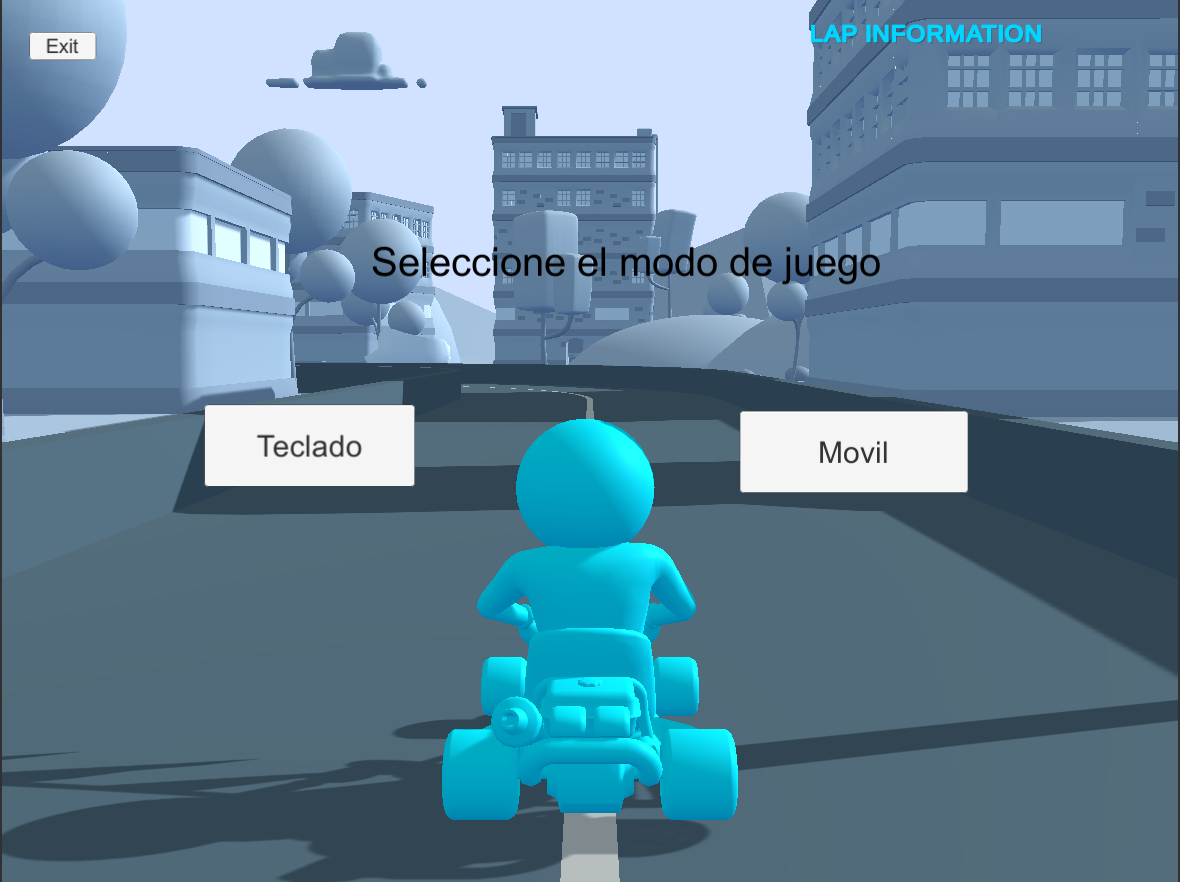
\includegraphics[width=0.5\textwidth]{./Imagenes/Bitmap/Menu_Principal_Juego}
     }
     \hfill
     \subfloat[Ejemplo de mando en Android\label{}]{%
       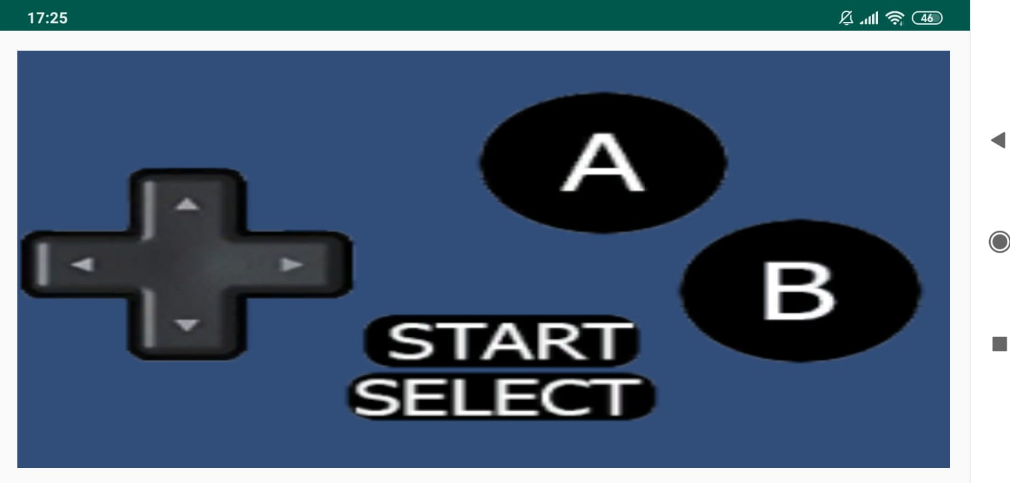
\includegraphics[width=0.5\textwidth]{./Imagenes/Bitmap/Mando}
     }
     \label{fig:quinta}
   \end{figure}


%-------------------------------------------------------------------
\section{Objetivos y organizaci\'on de las pruebas}
%-------------------------------------------------------------------

Previo a las pruebas con usuarios se definieron una serie de objetivos que cubrir durante la evaluaci\'on. Estos objetivos son los siguientes:

\begin {itemize}
\item Comprobaci\'on del funcionamiento de ambas aplicaciones (Android y Unity) en diferentes configuraciones.
\item Rendimiento de la parte de red, sobretodo en el env\'io de im\'agenes y el tiempo de env\'io de las pulsaciones.
\item Valorar la intuitividad del uso de la herramienta.
\end {itemize}

Para comprobar si el rendimiento de los diferentes procesos que realizan las aplicaciones para comunicarse se han implementado rastreadores o \textit{trackers} en las aplicaciones. Estos \textit{trackers} son clases y m\'etodos cuya funci\'on es la de llevar la cuenta del tiempo que tardan cada una de las diferentes acciones que se realizan. Se ha implementado un \textit{tracker} que se encarga de comenzar a contar cuando el usuario realiza una pulsaci\'on y para de contar una vez la aplicaci\'on recibe el mensaje de vibraci\'on. Este proceso es un ciclo completo de interacci\'on de usuario, lo que nos permite comprobar cu\'anto es el retardo que experimenta el usuario al interactuar.\\

Adem\'as de este \textit{tracker}, se han implementado 2 m\'as para controlar la compresi\'on y la descompresi\'on del PNG. La compresi\'on del PNG se realiza en Unity y la descompresi\'on se realiza en Android. Estos datos son recolectados en el juego y plasmados en un documento de texto para su posterior tratamiento. Estos datos nos ayudar\'an a saber cu\'anto tarda el frame desde que es recogido por la c\'amara en Unity hasta que es descomprimido y plasmado al usuario en el m\'ovil. \\

Estos procesos son dependientes del \textit{hardware} del m\'ovil y del ordenador ya que se utilizan varios hilos de ejecuci\'on de manera simult\'anea y el trabajo de compresi\'on y descompresi\'on del PNG requiere de un tiempo que puede incrementar si el procesador trabaja a frecuencias demasiado bajas. Es por esto que los \'ultimos datos que el \textit{tracker} extrae del usuario son el modelo de procesador, tarjeta gr\'afica y memoria RAM del ordenador. Para los datos del dispositivo m\'ovil se le pide al usuario que lo indique en un formulario posterior a la prueba.\\

El proceso de la prueba es igual para todos los usuarios pero sin demasiadas restricciones ya que lo que se pretende con esta prueba es que el usuario pruebe la herramienta jugando. Al extraer los datos mientras el usuario juega, no importa c\'omo juegue el usuario ni que pruebe una mec\'anica en espec\'ifico. El \'unico requisito es que la conexi\'on se cierre de manera por lo menos una vez por usuario ya que es en este momento cuando el m\'ovil env\'ia los datos recogidos por el \textit{tracker} al ordenador para realizar el documento de texto con los datos almacenados. Las pautas para la realizaci\'on de las pruebas han sido las siguientes:

\begin {itemize}
\item Se ha informado al usuario de los datos t\'ecnicos que se van a extraer de esta prueba (modelo de tarjeta gr\'afica, modelo de procesador, memoria RAM) y del posterior formulario a rellenar.
\item Se ha subido el ejecutable y el APK a un repositorio p\'ublico para que el usuario pueda hacer las pruebas.
\item Se ha indicado al usuario que el ordenador y el m\'ovil deben estar conectados a la misma red WIFI.
\item Se ha utilizado la aplicaci\'on de \textbf{Discord} para realizar una llamada con el usuario y que este compartiese la pantalla donde se estaba ejecutando el juego.
\item Se ha explicado al jugador que tiene que escanear el c\'odigo QR que aparece en el juego con la aplicaci\'on que se ha descargado del repositorio.
\item Se ha indicado al usuario que debe dar varias vueltas al circuito para que los datos puedan recogerse. 
\item Se ha realizado una entrevista con el usuario de entre 5 y 10 minutos para rellenar el formulario y comentar cualquier tipo de \textit{feedback} sobre la herramienta y el juego.
\end {itemize}

Al final de la prueba se realiza una charla con el usuario donde este nos indica todas las observaciones, sugerencias de mejora y puntos positivos. En esta charla tambi\'en se hacen algunas preguntas como por ejemplo el modelo de m\'ovil con el que ha realizado la prueba, experiencia jugando a videojuegos y cuales juega normalmente, opini\'on sobre la fluidez de la prueba y el \textit{feedback} recibido (visual y h\'aptico gracias a la vibraci\'on). 

%-------------------------------------------------------------------
\section{Resultados de las pruebas}
%-------------------------------------------------------------------


\begin{table}[h]
    \begin{tabular}{ccccc}
        \toprule
         \textbf{Usuarios} & \textbf{M\'ovil} & \textbf{Procesador} & \textbf{RAM} & \textbf{Gr\'afica} \\
        \midrule
\textbf{Usuario 1} & One Plus 6 & i7-5820K 3.30GHz & 32GB &  GTX 980\\
\textbf{Usuario 2} & One Plus 6 & i7-6700K 4.0GHz & 16GB &  GTX 1080 \\
\textbf{Usuario 3} & S9+ & i7-6700HQ 2.6GHz & 16GB &  GTX 960M \\
\textbf{Usuario 4} & S8 & A10-5800K 3.8GHz & 8GB & Radeon 7660D \\
\textbf{Usuario 5} & S9+ & i7-6800K 3.4GHz & 32GB &  GTX 1080 \\
        \bottomrule
    \end{tabular}
\caption{Sistemas utilizados por cada usuario durante las pruebas}
\label{tablausuarios}
\end{table}


% Variable local para emacs, para  que encuentre el fichero maestro de
% compilaci�n y funcionen mejor algunas teclas r�pidas de AucTeX
%%%
%%% Local Variables:
%%% mode: latex
%%% TeX-master: "../ManualTeXiS.tex"
%%% End:
